% Created 2021-04-20 mar. 23:02
% Intended LaTeX compiler: pdflatex
\documentclass[11pt]{article}
\usepackage[utf8]{inputenc}
\usepackage[T1]{fontenc}
\usepackage{graphicx}
\usepackage{grffile}
\usepackage{longtable}
\usepackage{wrapfig}
\usepackage{rotating}
\usepackage[normalem]{ulem}
\usepackage{amsmath}
\usepackage{textcomp}
\usepackage{amssymb}
\usepackage{capt-of}
\usepackage{hyperref}
\author{Bouton Nicolas}
\date{April 2021}
\title{Rapport du Projet Hybrid d'APP}
\hypersetup{
 pdfauthor={Bouton Nicolas},
 pdftitle={Rapport du Projet Hybrid d'APP},
 pdfkeywords={},
 pdfsubject={},
 pdfcreator={Emacs 27.1 (Org mode 9.3)}, 
 pdflang={English}}
\begin{document}

\maketitle
\tableofcontents

Le but du projet était de paralléliser un programme séquentielle de \textbf{gradient
conjugué} avec une implémentation \textbf{hybrid MPI / Pthread}.

\section{Réduction d'une somme hybride MPI / Pthread}
\label{sec:org21f221b}
\subsection{Schéma expliquant la démarche prise}
\label{sec:orgf763a4d}

\begin{figure}[htbp]
\centering
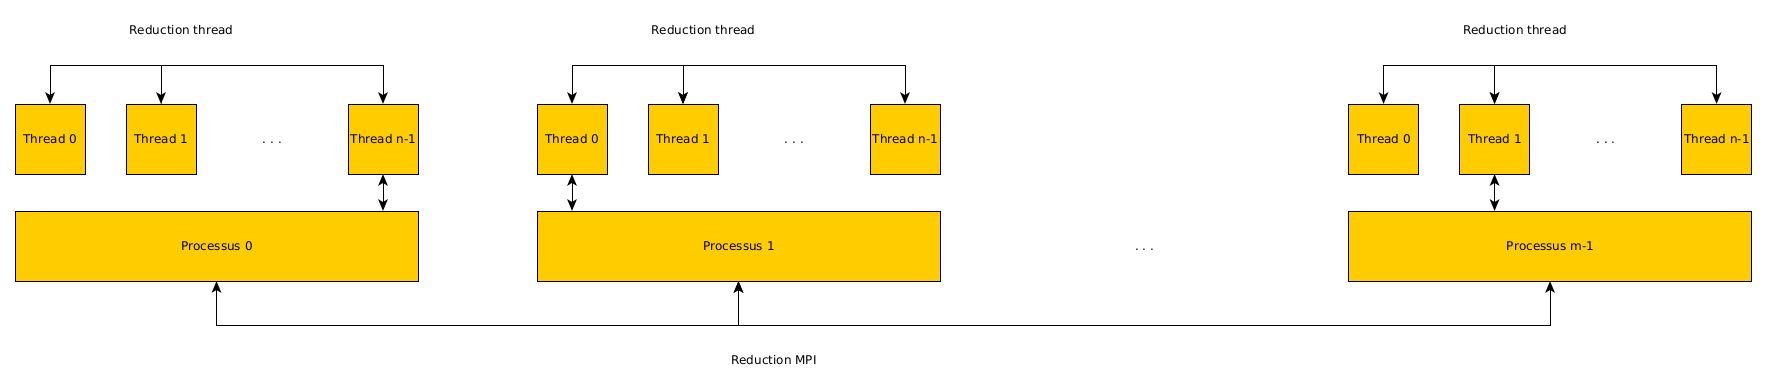
\includegraphics[width=300px]{../ressources/hyb_reduc.png}
\caption{\label{fig:org1340d85}Schéma expliquant la démarche prise}
\end{figure}

\subsection{Explication du code}
\label{sec:org699ec20}

Mon raisonnement est le suivant:
\begin{enumerate}
\item Chaque thread de chaque processus MPI va sommer sa valeur avec celle qu'il
partage avec ces autres threads en commun (du même processus MPI)
\item Une fois que la somme est faites localement sur chaque processus MPI, on
élit un thread pour qu'il fasse la réduction avec les autres threads élus
des autres processus MPI. Par exemple pour le \textbf{processus 0}, c'est le
thread \textbf{n-1} qui est élu alors que pour le \textbf{processus 1} c'est le \textbf{0}. En
réalité c'est le premier thread qui finit qui est élu.
\item Une fois que les threads élu ont fait leur réduction ensembles. Il faut
que les autres threads non élu actualisent leurs réductions.
\end{enumerate}


Pour ce faire j'ai utilisé un \textbf{sémaphore} pour pouvoir élire le premier
thread qui arrive. Et à la fin pour l'actualisation du résultat on pourait
lâcher tout les threads en faisant que le threads élu fasse une boucle de
\textbf{sem\textsubscript{post}} mais je ne sais pas pourquoi ca ne marchais pas. Donc j'ai laisser
l'actualisation en séquentielle.

A la fin de la fonction, j'ai mis une \textbf{barrière} pour pouvoir synchroniser
tout les threads de tout les processus MPI, en mettant d'abord une barrier au
niveau des threads du même processus pui une barrier entre touts les
processus (qui est prise \textbf{NUM\textsubscript{THREADS}} fois car je ne sais pas trop comment
faire pour qu'un seul thread le fasse sachant que nous n'avons pas l'id du
thread).

Et j'ai aussi fait attention de remettre les variables de la structure comme
elles étaient initialisés pour le prochain tour de boucle. (je fais donc un
\textbf{sem\textsubscript{post}} pour le dernier threads afin que le premier thread qui arrrive
dans le \textbf{sem\textsubscript{wait}} passe).

\section{Echange point à point hybrides MPI / Pthread}
\label{sec:org616f4b8}

Pour ce qui est des échanges point à point, cela est relativement la même
chose que pour la réduction. Il y 2 grandes parties:
\begin{enumerate}
\item Echanges entre les threads élu des processus MPI (premier arrivé)
\item Actualisation entre les threads du même processus MPI avec les valeurs que
le thread élu à échangé.

La aussi j'ai utilisé un \textbf{sémaphore} pour élire le premier thread. Et comme
pour la réduction hybride j'ai fait attention à réinitialisé les variables
pour le dernier thread.
\end{enumerate}

\section{Algorithme du gradient conjugué parallèle MPI / Pthread}
\label{sec:org1025fb1}
\subsection{Initialisation}
\label{sec:org200af86}

La seule chose à prendre en considération c'est que c'est le premier thread
du premier processus MPI qui contient la valeur du \textbf{i global} égale à \textbf{0}.

Et que c'est le dernier thread du dernier processus MPI qui contient la
valeur \textbf{i global} égale à \textbf{i global maximum} du tableau.

\subsection{Réduction}
\label{sec:org52daf44}

Il y a 2 fonction qui font une réduction:
\begin{itemize}
\item le calcul de la norme au carré
\item le rapport de 2 profuits scalaire
\end{itemize}


En réalisté ce sont toutes les fonctions qui font une réduction en
séquentielle et qui retourne un flottant.

Donc pour ces 2 fonctions j'ai utilisé la fonction de réduction hybride.

\subsection{Produit matrice vecteur}
\label{sec:orgb690564}

A faire.

\section{Conclusion}
\label{sec:org50dd064}

Comme vous allez le voir à l'exécution, mon implémentation donne un résultat
faux mais je ne comprends pas pourquoi. Si jamais vous avez un retour sur mon
implémentation ou mon raisonnement je suis prenneur.
\end{document}
